\documentclass[10pt,letterpaper]{article}

\usepackage[utf8]{inputenc}
\usepackage[spanish,es-nodecimaldot]{babel}
\usepackage{amsmath}
\usepackage{amssymb}
\usepackage{graphicx}
\usepackage{mathtools}

\usepackage{multicol}

\usepackage{enumitem}

\newcommand{\ihat}{\hat{\textbf{\i}}}
\newcommand{\jhat}{\hat{\textbf{\j}}}
\newcommand{\uhat}{\hat{\textbf{u}}}
\DeclarePairedDelimiter{\norm}{\lVert}{\rVert}

\usepackage[top=1in, bottom=1in, left=1in, right=1in]{geometry}


\begin{document}

\begin{titlepage}
    \centering

    {\scshape\LARGE Universidad Nacional Autónoma de México \par}

    \vspace{1cm}
    {\scshape\Large Facultad de Ciencias\par}
    \vspace{1.5cm}

    \begin{center}
        
\includegraphics[scale=.1]{../../assets/img/logo.png}
    \end{center}

    \vspace{.8 cm}

    {\LARGE Tarea 02: \par}
    {\huge\bfseries Convexidad, vecindarios, búsqueda local: Hill Climbing y Búsqueda Tabú \par}

    \vspace{0.5cm}
    \large{\itshape{Pablo A. Trinidad Paz}} \small{ - 419004279}

    \vfill

    Trabajo presentado como parte del curso de
    \textbf{Cómputo Evolutivo}
    impartido por el profesor \textbf{Mario Iván Jaen Márquez}. \par
    \vspace{0.5cm}
    Fecha de entrega: \textbf{22 de Febrero de 2019}.
\end{titlepage}

\section{Teoría}
    \small{*Código utilizado en Jupyter Notebook \textbf{\textit{Theory.ipynb}}}

    \begin{enumerate}
        \item Sean $f_2, f_2: \mathbb{R} \rightarrow \mathbb{R}$ dadas por
            \begin{equation*} \begin{split} \begin{aligned}
                f_1(x) &= x^2 - 2ex + e^2 - 2, \\
                f_2(x) &= x^6 - 6ex^5 + 15e^2x^4 - 20e^3x^3 + 15e^4x^2 - 6e^5x + e^6 - 6 \\
            \end{aligned} \end{split} \end{equation*}

            \begin{enumerate}
                \item Demuestre que $f_1$ y $f_2$ son funciones convexas \\

                    \textbf{Solución:}

                    Una función $f$ es convexa si se cumple que:
                    \begin{equation*} \begin{split} \begin{gathered}
                        \forall x, y \in Dom(f)  \text{ y } \forall a \in [0, 1] \\
                        f(ax + (1-a)y) \leq af(x) + (1 - a)f(y).
                    \end{gathered} \end{split} \end{equation*}
                    Además, se cumple que si la función es doblemente derivable
                    (y de una sola variable) es convexa en un intervalo sí y solo sí
                    su segunda derivada no es negativa.

                    Para $f_1(x)$:
                    \begin{equation*} \begin{split} \begin{gathered}
                        f_1'(x) = 2x - 2e \\
                        f_1''(x) = 2 \\
                        \Rightarrow f_1''(x) > 0 \\
                        \therefore \; f_1 \text{ es convexa} \quad \blacksquare
                    \end{gathered} \end{split} \end{equation*}

                    Para $f_2(x)$:
                    \begin{equation*} \begin{split} \begin{gathered}
                        f_2'(x) =  6 x^5  - 30 e x^4  + 60 e^2 x^3  - 60 e^3 x^2 + 30 e^4 x - 6 e^5  \\
                        f_2''(x) = 30 x^4 - 120 e x^3 + 180 e^2 x^2 - 120 e^3 x  + 30 e^4 \\
                        f_2''(x) = 30(e - x)^4 \\
                        \Rightarrow f_2''(x) > 0 \\
                        \therefore \; f_2 \text{ es convexa} \quad \blacksquare
                    \end{gathered} \end{split} \end{equation*}

                \item Utilice el algoritmo del descenso por gradiente implementado
                para minimizarlas. Use $x_0 = 0$ como punto inicial y $\alpha$
                arbitrario. ¿Qué valores de $\alpha$ hacen más eficiente el algoritmo
                para cada función? \\

                    \textbf{Solución:}

                    Para responder a la pregunta anterior se corrió el
                    descenso por gradiente con múltiples valores de $\alpha$
                    y se determinó que el valor de $\alpha$ más eficiente sería
                    aquel que lograra encontrar un óptimo en el menor número
                    de iteraciones. Para saber si el valor óptimo obtenido
                    a partir de dicha $\alpha$ era aceptable, se calculó la
                    desviación estándar, promedio y media de los resultados
                    de cada prueba. \\

                    Para ambas funciones, el gradiente corrió bajo los
                    siguientes parámetros:

                        \begin{itemize}
                            \item Precisión: $1 \times 10^{-8}$
                            \item Número máximo de iteraciones: $10^{10}$
                        \end{itemize}

                    \clearpage

                    \textbf{Resultados de $f_1$}:

                    \begin{center}
                        Valores de $\alpha$ para la función $f_1$ \\
                        \begin{tabular}{c|r|l} 
                            \hline
                            \multicolumn{1}{|c|}
                            {$\alpha$} & \textbf{Número de iteraciones} & \multicolumn{1}{l|}{\textbf{Valor mínimo}}  \\ 
                            \hline
                            0.000005    &    790773    &    2.71728184 \\
                            0.00001    &    430042    &    2.71778184 \\
                            0.00005    &    102100    &    2.71818185 \\
                            0.0001    &    54513    &    2.71823184 \\
                            0.0005    &    12508    &    2.71827184 \\
                            0.001    &    6598    &    2.71827684 \\
                            0.005    &    1476    &    2.71828085 \\
                            0.01    &    769    &    2.71828134 \\
                            0.05    &    164    &    2.71828174 \\
                            0.1    &    81    &    2.71828179 \\
                            0.5    &    2    &    2.71828183 \\
                        \end{tabular}
                    \end{center}

                    \begin{multicols}{2}
                        \begin{center}
                            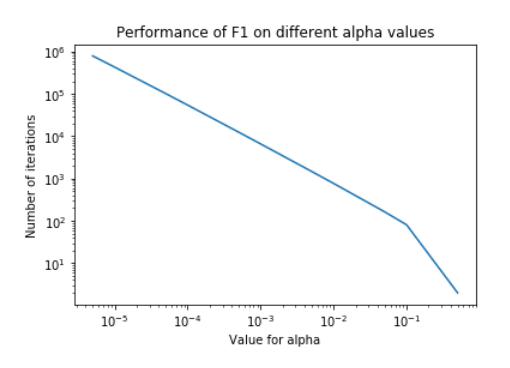
\includegraphics[scale=.4]{assets/theory/1-b/f1-performance.png}
                        \end{center}
                        \begin{center}
                            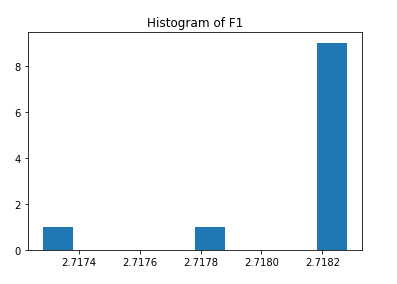
\includegraphics[scale=.5]{assets/theory/1-b/f1-dist.png}
                        \end{center}
                    \end{multicols}

                    Con una desviación estándar $\sigma \approx 0.000303$,
                    promedio $\mu \approx 2.7181303273$ y media $\approx 2.7182768400$
                    se puede concluir de forma segura que el valor óptimo de $\alpha$ para
                    $f_1$ es \textbf{0.5} y que el mínimo se encuentra en
                    $x=2.718281828459045$.

                    \begin{center}
                        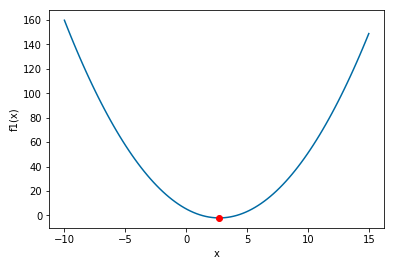
\includegraphics[scale=.6]{assets/theory/1-b/f1-minimum.png}
                    \end{center}

                    \clearpage

                    \textbf{Resultados de $f_2$}:
                    \begin{center}
                    Valores de $\alpha$ para la función $f_2$ \\
                    \begin{tabular}{c|r|l} 
                        \hline
                        \multicolumn{1}{|c|}
                        {$\alpha$} & \textbf{Número de iteraciones} & \multicolumn{1}{l|}{\textbf{Valor mínimo}}  \\ 
                        \hline
                            5e-06    &    5266300    &    2.45496429845281 \\
                            1e-05    &    4691757    &    2.4836925848909828 \\
                            5e-05    &    3587912    &    2.538885692619941 \\
                            0.0001    &   3196467    &    2.5584580445544773 \\
                            0.0005    &   2444410    &    2.59606066860143 \\
                            0.001    &    2163480    &    2.60939515596596 \\

                        \end{tabular}
                    \end{center}

                    \begin{multicols}{2}
                        \begin{center}
                            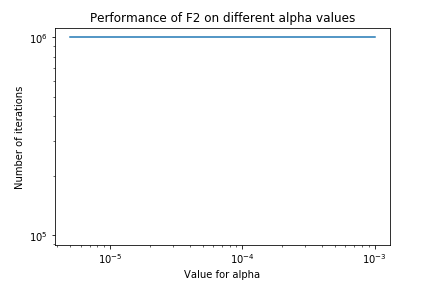
\includegraphics[scale=.45]{assets/theory/1-b/f2-performance.png}
                        \end{center}
                        \begin{center}
                            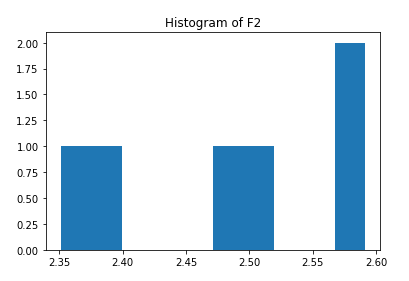
\includegraphics[scale=.45]{assets/theory/1-b/f2-dist.png}
                        \end{center}
                    \end{multicols}

                    Con una desviación estándar $\sigma \approx 0.0558$,
                    promedio $\mu \approx 2.5402427408$ y media $\approx 2.5486718686$
                    Se puede utilizer \textbf{el valor más óptimo de} $\alpha = 0.001$ y
                    su mínimo hallado $x=2.60939515596596$ ya que se encuentra dentro de
                    $[\sigma - \mu, \sigma + \mu]$.

                    \begin{center}
                        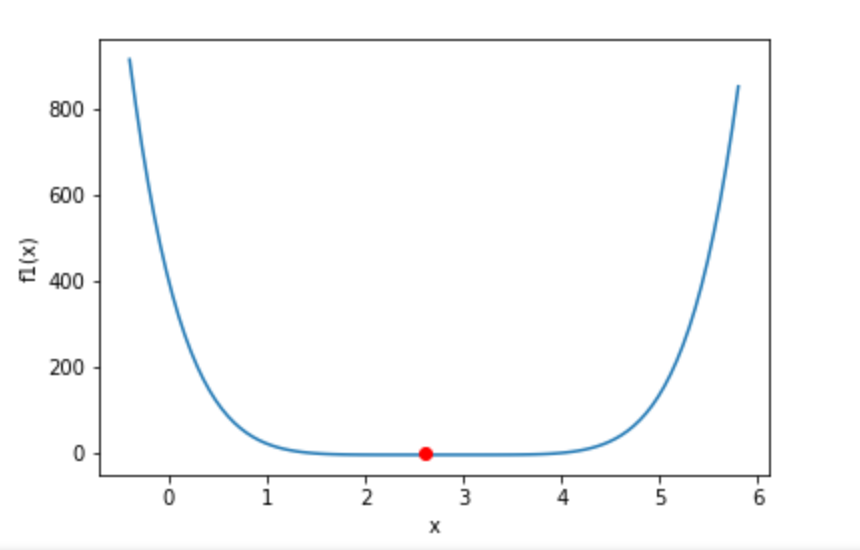
\includegraphics[scale=.6]{assets/theory/1-b/f2-minimum.png}
                    \end{center}

                    \clearpage

            \end{enumerate}

        \item Lea el capítulo 1 del siguiente libro para resolver las preguntas de
              esta sección:
        
            \textit{Z. Michalewicz et al., How to Solve It: Modern Heuristics. Springer Berlin Heidelberg 2004}

            \begin{enumerate}
                \item Mencione al menos 2 razones por las cuales un problema del
                      mundo real puede no ser resuelto fácilmente. NO USE ninguna
                      de las razones enumeradas en la página 11 del capítulo 1.
                      \begin{itemize}
                          \item Algunos problemas son tan complejos que obtener
                                un modelo que contemple todos sus aspectos puede
                                ser muy complicado. Por otro lado, dado un modelo
                                detallado del problema, derivar una solución óptima
                                puede ser extremadamente complicado.
                                Usualmente se reduce a dos opciones: 1. Modelar el
                                problema contemplando todos los aspectos y obtener una
                                solución aproximada usando métodos no convencionales
                                o 2. Aproximar un segundo modelo que imite las
                                características del problema y obtener una solución
                                exacta a ese modelo aproximado por métodos convencionales.
                                \begin{equation*} \begin{split} \begin{gathered}
                                    \text{1) }\mathrm{Problem} \implies \mathrm{Model_a} \implies \mathrm{Solution_p}(\mathrm{Model_a}) \\
                                    \text{2) }\mathrm{Problem} \implies \mathrm{Model_p} \implies \mathrm{Solution_a}(\mathrm{Model_p})
                                \end{gathered} \end{split} \end{equation*}
                          \item \textbf{Los problemas cambian con el tiempo}. Si derivar un modelo
                                (de cualquier tipo) al problema fue costoso y no contempla
                                que la naturaleza del problema cambió mientras se derivaba,
                                éste puede terminar siendo obsoleto. Además, existe otra
                                complicación: \textbf{las limitantes del problema}. Las
                                limitantes, aunque pueden reducir el tamaño del espacio
                                de búsqueda, suelen terminar agregando más complejidad
                                al modelo ya que no todas las posibles soluciones cumplirán
                                necesariamente con las limitantes.
                      \end{itemize}

                \item Supongamos que la optimización de una función $f$ requiere de
                      10 variables de decisión $x_i(i = 1,...,10)$, cada una de las
                      cuales está en el dominio $-50 \leq x_i \leq 50$.
                      \begin{itemize}
                        \item Si $x_i$ puede tomar solo valores enteros ¿cuál
                              es el tamaño del espacio de búsqueda de este problema? \\

                              \textbf{Soluución:}
                              Existen 101 enteros en el rango $[-50, 50]$, por lo tanto
                              hay $101^{10}$ combinaciones posibles. \\

                        \item Si $x_i$ puede tomar valores reales y se usa
                              una precisión de ocho lugares decimales ¿cuál
                              es el tamaño del espacio de búsqueda del problema?
                              \textbf{Soluución:}

                              \textbf{Soluución:}
                              Existen $10^8$ números decimales entre cada entero
                              (incluyéndolo) y hay 101 enteros disponibles en el
                              rango propuesto, es decir, hay $101 \times 10^8$
                              valores disponibles, por lo tanto hay 
                              $(101 \times 10^8)^{10} \approx 1.1 \times 10^{100}$
                              combinaciones.
                      \end{itemize}
            \end{enumerate}

        \item Investiga a qué se refieren los términos: \textbf{exploración}
              y \textbf{explotación} dentro de las fases de un algoritmo evolutivo. \\
        
            \begin{enumerate}
                \item \textbf{Exploración} (exploration): Suele ser usado para
                      referirse a buscar en todo el espacio de búsqueda una
                      solución candidata al problema.
                \item \textbf{Explotación} (exploitation): Suele ser usado para
                      referirse a buscar una nueva solución en una región limitada
                      del espacio de búsqueda al rededor de una solución ya existente.
            \end{enumerate}

        \item ¿Considerarías al algoritmo \textit{hill climbing} un \textit{greedy algorithm}?
              ¿Por qué? \\

              \textbf{Solución:} Sí. Los algoritmos greedy son conocidos por encontrar
              soluciones "parcialmente buenas", en otras palabras, óptimos locales, y
              aunque \textit{hill climbing} pueda encontrar óptimos globales en funciones
              convexas, para otro tipo de funciones terminará convergiendo en un óptimo
              local, es decir, las soluciones ya no podrán mejorar dentro de su vecindario
              local.

        \clearpage

        \item Considera la función $f(x) = x^2 + 3x + 5$ definida sobre los enteros
              $\mathbb{Z}$ en el intervalo $[-20, 20]$. Vamos a usar el algoritmo
              \textit{hill climbing} para encontrar el valor de $x$ que minimiza
              la función en ese intervalo.

              \begin{enumerate}
                  \item Grafica la función
                        \begin{center}
                            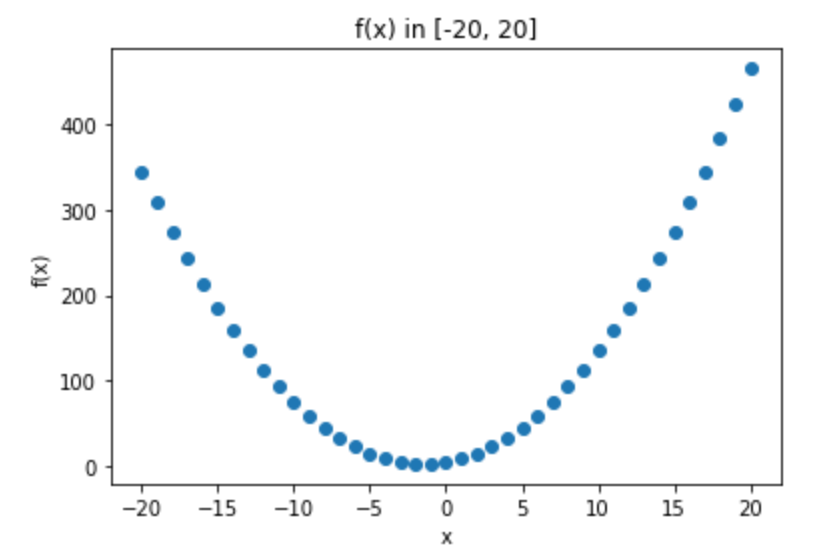
\includegraphics[scale=.5]{assets/theory/5-a/f-plot.png}
                        \end{center}
                  \item Considera el vecindario definido por
                  $N(x) = {x + 1, x - 1} \; \forall x \; \in \; [-19, 19]$. Usa
                  como solución inicial $x_0=6$ e indica los valores que toma
                  $x_t$ y $f(x_t)$ en cada iteración $t$ del algoritmo.
              \end{enumerate}

              \begin{multicols}{2}
                \begin{center}
                    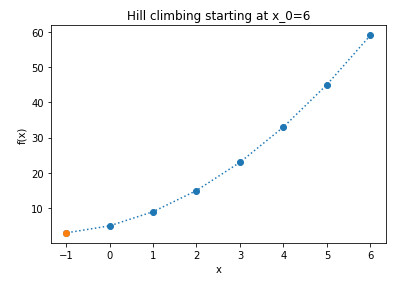
\includegraphics[scale=.5]{assets/theory/5-b/hill-climb.png}
                \end{center}
                \begin{center}
                    \begin{tabular}{|c|c|c|} 
                        \hline
                        \multicolumn{1}{|c|}
                        {$t$} & $x_t$ & \multicolumn{1}{l|}{ $f(x_t)$ }  \\ 
                        \hline \hline
                            1 & 6 & 59 \\ \hline
                            2 & 5 & 45 \\ \hline
                            3 & 4 & 33 \\ \hline
                            4 & 3 & 23 \\ \hline
                            5 & 2 & 15 \\ \hline
                            6 & 1 & 9 \\ \hline
                            7 & 0 & 5 \\ \hline
                            8 & -1 & 3 \\ \hline
                    \end{tabular}
                \end{center}
              \end{multicols}
    \end{enumerate}

\section{Práctica}
    Solución en Jupyter Notebook \textbf{\textit{PSet.ipynb}}

    \begin{enumerate}
        \item Con $V_1$ se econtró $x^* = (0.0, -5.0)$ el cual resulta en $F(x^*)=-54.6875$
        \item Con $V_{\infty}$ se econtró $x^* \approx (5.6, 5.7)$ el cual resulta en $F(x^*) \approx -191.995608$
    \end{enumerate}
\end{document}
